\chapter{Auswertung Benchmark}
Im folgenden werden die Ergebnisse des Benchmarks ausgewertet.
Dazu wird zu erst die Gesamtlaufzeit des Benchmarks in \autoref{auswertung:generell} analysiert. Dabei wird zwischen zeilenbasierten und spatenbasierten
Tabellen unterschieden.
Anschließend wird in \autoref{auswertung:queries} auf die Laufzeit der
einzelnen Unterabfragen des Benchmarks eingegangen.
Dabei soll untersucht werden welche Abfragen besonders schnell sind.
In \autoref{auswertung:basic_indizes} und \autoref{auswertung:hardware}
wird der Einfluss von Indizes bzw.\ unterschiedlicher Hardwarekonfigurationen
untersucht.

\section{Gesamtlaufzeit des Benchmarks}\label{auswertung:generell}

\begin{tabularx}{\textwidth}{|X|r|r|}
	\toprule
	 & \textbf{Rowstore} & \textbf{Columnstore}\\
	\midrule
	\endhead
	\hline
	\caption{Gesamtlaufzeiten von Row- und Columnstore in usec}
	\label{auswertung:gesamtlaufzeit}
	\endfoot
	Durchschnitt & 754689 & 3591003 \\
	Minimum & 725710 & 3451791 \\
	Maximum & 858595 & 4079505 \\
	Median & 752236 & 3577376 \\
	Standardabweichung & 17619 & 79002\\
	Gesamt & 754689 & 3591003 \\
\end{tabularx}

Allgemein sollten Benchmarks auf der HANA Datenbank immer zwischen
Row- und Columnstore unterscheiden.
Dies wird deutlich beim Betrachten der Allgemeinen Laufzeit.
Wie \autoref{auswertung:gesamtlaufzeit} zu entnehmen ist, besteht ein deutlicher
Unterschied in der Laufzeit zwischen Row- und Columnstore.
Da der SSBM Benchmark als Maß für Abfragen im Bereich des Datawarehouse
eingesetzt wird, kann also allgemein gesagt werden,  dass der Columnstore
dem Rowstore im Datawarehouse Umfeld vorzuziehen ist.
Jedoch sollte bedacht werden, dass es sich bei dem SSBM Benchmark um
reine Abfragen von Daten handelt. Wie in \autoref{row_col:rowstore} beschrieben
kann ein Rowstore von Vorteil sein, wenn Daten gespeichert werden.

\begin{figure}[H]
	\centering
	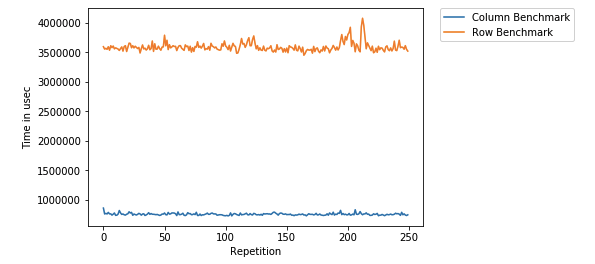
\includegraphics[width=0.7\textwidth]{images/performanceentwicklung.png}
	\caption{Gesamtlaufzeit von Row- und Columnstore}\label{auswertung:gesamtlaufzeit:graph}
\end{figure}
Anhand der Standardabweichung und \autoref{auswertung:gesamtlaufzeit:graph} ist auch zu sehen, dass der Columnstore
eine konstantere Zeit pro Abfrage aufweist.
Allerdings da der Rowstore im allgemeinen langsamer ist als der Columnstore
kann dies vernachlässigt werden, da die Standardabweichung relativ zur
Gesamtlaufzeit sehr gering ist.

\section{Vergleich der SSBM Queries}\label{auswertung:queries}

Im folgenden werden die einzelnen Queries des SSBM Benchmarks separat betrachtet.

%TODO
% Vergleich von q1, q2, q3, q4 etc.
% Diagramm
% Welche ist die schnellste und warum?
% Stabilität einzelner Queries


\section{Einfluss der grundlegenden Indizes}\label{auswertung:basic_indizes}

%TODO
% Row with or without indices
% Column with or without indices

\section{Auswirkung unterschiedlicher Hardwarekonfiguration}\label{auswertung:hardware}

%TODO
% Beschreibe setup bsp 4GB ram, 2CPU etc.
% Gibt es einen effekt?
% Wenn ja isolieren und begründen

\section{Vergleich zu anderen Datenbanksystemen}\label{auswertung:vergleich}

%TODO
%https://github.com/Osslack/HANA_SSBM/issues/27
%siehe auch ressourcen

